\documentclass[aspectratio=169]{beamer}
\usepackage[utf8]{inputenc}\usepackage[T1]{fontenc}\usepackage{lmodern}
\usetheme{Madrid}
\setbeamertemplate{navigation symbols}{}
\setbeamercovered{transparent}
\setbeamertemplate{itemize items}[circle]
\setbeamertemplate{enumerate items}[default]
\setlength{\parskip}{0.25em}
\definecolor{UNBCDark}{RGB}{0,74,37}
\definecolor{UNBCGold}{RGB}{189,155,96}
\definecolor{SoftGray}{RGB}{244,246,248}
\definecolor{AccentRed}{RGB}{192,57,43}
\definecolor{AccentBlue}{RGB}{41,98,255}
\definecolor{AccentTeal}{RGB}{0,150,136}
\definecolor{AccentOrange}{RGB}{230,126,34}
\setbeamercolor{normal text}{fg=black,bg=white}
\setbeamercolor{structure}{fg=UNBCDark}
\setbeamercolor{title}{fg=white,bg=UNBCDark}
\setbeamercolor{subtitle}{fg=UNBCGold}
\setbeamercolor{frametitle}{fg=white,bg=UNBCDark}
\setbeamercolor{block title}{fg=white,bg=UNBCDark}
\setbeamercolor{block body}{fg=black,bg=SoftGray}
\setbeamercolor{block title alerted}{fg=white,bg=AccentRed}
\setbeamercolor{block body alerted}{fg=black,bg=SoftGray}
\setbeamercolor{item}{fg=UNBCDark}
\setbeamercolor{alerted text}{fg=AccentRed}
\setbeamercolor{author in head/foot}{fg=white,bg=UNBCDark}
\setbeamercolor{date in head/foot}{fg=white,bg=UNBCDark}
\usepackage{booktabs,multirow,array,amsmath,amssymb,bm,graphicx,adjustbox}
\usepackage{tikz,pgfplots,multicol,tcolorbox,hyperref}
\tcbuselibrary{skins}
\pgfplotsset{compat=1.18}
\usetikzlibrary{arrows.meta,positioning,calc,decorations.pathreplacing}
\hypersetup{colorlinks=true,linkcolor=UNBCDark}
\setbeamertemplate{headline}{}
\setbeamertemplate{footline}{%
  \leavevmode\hbox{%
  \begin{beamercolorbox}[wd=.78\paperwidth,ht=2.8ex,dp=1.2ex,leftskip=1em]{author in head/foot}%
  \color{white}\textbf{ECON 308} \hspace{0.4em}\textcolor{UNBCGold}{|}\hspace{0.4em}International Economic Relations%
  \end{beamercolorbox}%
  \begin{beamercolorbox}[wd=.22\paperwidth,ht=2.8ex,dp=1.2ex,rightskip=1em plus1fil]{date in head/foot}%
  \color{white}\insertframenumber/\inserttotalframenumber%
  \end{beamercolorbox}}%
}
\newtcolorbox{insight}[1]{colback=UNBCGold!12,colframe=UNBCGold!70!black,
  title={\small\bfseries #1},left=1.5mm,right=1.5mm,top=0.8mm,bottom=0.8mm,boxrule=0.5pt,arc=2mm}
\newtcolorbox{canadex}[1][Canadian Example]{colback=AccentTeal!9,colframe=AccentTeal,
  title={\small\bfseries #1},left=1.5mm,right=1.5mm,top=0.8mm,bottom=0.8mm,boxrule=0.5pt,arc=2mm}
\newtcolorbox{discuss}{colback=AccentBlue!8,colframe=AccentBlue,
  title={\small\bfseries Discussion},left=1.5mm,right=1.5mm,top=0.8mm,bottom=0.8mm,boxrule=0.5pt,arc=2mm}
\newtcolorbox{varbox}{colback=SoftGray,colframe=UNBCDark!50,
  left=1.5mm,right=1.5mm,top=0.8mm,bottom=0.8mm,boxrule=0.4pt,arc=2mm}
\newcommand{\FIG}[1]{\begin{center}%
  \includegraphics[width=\textwidth,height=0.68\textheight,keepaspectratio]{#1}%
  \end{center}}
\newcommand{\FIGH}[2][0.85]{\begin{center}%
  \includegraphics[width=#1\textwidth,height=0.72\textheight,keepaspectratio]{#2}%
  \end{center}}

\title{\textbf{Economies of Scale, Imperfect Competition, and International Trade}}
\subtitle{{\large ECON 308 -- International Economic Relations \quad Chapter 7}}
\author{Muhebullah Karimzada}
\institute{School of Economics \\ University of Northern British Columbia}
\date{Fall 2026}

\begin{document}

\begin{frame}[plain]\titlepage\end{frame}

\begin{frame}{Opening Puzzle: Why Do Canada and Germany Both Export Cars?}
\begin{columns}
\begin{column}{0.57\textwidth}
\begin{itemize}
  \item Germany and Canada are both capital-abundant, high-income countries with similar technology.
  \item H-O predicts \emph{little} trade between them.
  \item \textbf{Reality}: Canada exports Chrysler minivans and Lincoln SUVs; Germany exports BMW and Mercedes.
  \item This is \textbf{intra-industry trade (IIT)}: simultaneously exporting and importing the same product category.
  \item The Ricardian and H-O models \emph{cannot explain} IIT. We need a new framework.
\end{itemize}
\end{column}
\begin{column}{0.40\textwidth}
\begin{insight}{New Insight Needed}
  When there are \emph{economies of scale} and \emph{product differentiation}, each country specialises in different \emph{varieties} of a good --- not different goods. Trade expands variety without eliminating production at home.
\end{insight}
\end{column}
\end{columns}
\end{frame}

\begin{frame}{Learning Objectives}
\begin{enumerate}
  \item Distinguish external from internal economies of scale and their implications.
  \item Derive the equilibrium in a monopolistically competitive industry.
  \item Show how trade expands the market and generates gains via the Krugman model.
  \item Measure intra-industry trade using the Grubel-Lloyd index.
  \item Explain why industrial clusters arise and exhibit path dependence.
  \item Evaluate the policy implications of economies of scale.
\end{enumerate}
\end{frame}

\begin{frame}{Economies of Scale: The Basic Concept}
\begin{columns}
\begin{column}{0.52\textwidth}
\begin{block}{Economies of Scale (EoS)}
  Average cost \emph{falls} as output rises: $AC(Q) = F/Q + c$, where $F$ is fixed cost and $c$ is constant marginal cost.
\end{block}
\vspace{0.3em}
\textbf{Why EoS arise:}
\begin{itemize}
  \item Fixed costs (R\&D, tooling, brand) spread over more units.
  \item Specialisation of labour and equipment at large scale.
  \item Indivisibilities: some technologies require minimum scale.
  \item Learning-by-doing: productivity rises with cumulative output.
\end{itemize}
\vspace{0.2em}
\textbf{Two types}: external (industry-level) and internal (firm-level).
\end{column}
\begin{column}{0.45\textwidth}
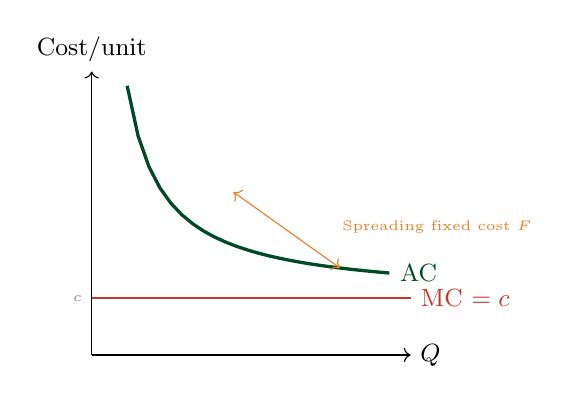
\begin{tikzpicture}[scale=0.9]
\draw[->] (0,0) -- (4.5,0) node[right]{\small $Q$};
\draw[->] (0,0) -- (0,4) node[above]{\small Cost/unit};
% AC curve: F/Q + c
\draw[UNBCDark,very thick,domain=0.5:4.2] plot(\x,{1.5/\x+0.8}) node[right]{\small AC};
% MC line
\draw[AccentRed,thick] (0,0.8) -- (4.5,0.8) node[right]{\small MC $=c$};
\draw[dashed,gray] (0,0.8) node[left]{\tiny $c$};
\draw[<->,AccentOrange] (2,2.3) -- (3.5,1.23);
\node[AccentOrange,right] at (3.4,1.8) {\tiny Spreading fixed cost $F$};
\end{tikzpicture}
\end{column}
\end{columns}
\end{frame}

\begin{frame}{External vs.\ Internal Economies of Scale}
\begin{columns}
\begin{column}{0.5\textwidth}
\begin{block}{External Economies of Scale}
  Average cost falls as the \emph{industry} grows, not the individual firm.\\[0.2em]
  Each firm remains small; market is competitive.\\[0.2em]
  Sources: shared labour pool, specialised suppliers, knowledge spillovers.
\end{block}
\vspace{0.3em}
\begin{block}{Internal Economies of Scale}
  Average cost falls as the \emph{firm} grows.\\[0.2em]
  Large firms can undercut small ones $\Rightarrow$ market becomes imperfectly competitive (monopoly, oligopoly, or monopolistic competition).
\end{block}
\end{column}
\begin{column}{0.47\textwidth}
\begin{adjustbox}{max width=\columnwidth}
\begin{tabular}{lll}
\toprule
\textbf{Type} & \textbf{Market} & \textbf{Example}\\
\midrule
External & Competitive & Vancouver mining\\
 & & (many small firms,\\
 & & cluster benefits all)\\
\midrule
Internal & Monopolistic & Automobile\\
 & competition & manufacturers\\
\midrule
Internal & Oligopoly & Aircraft (Boeing,\\
 & & Airbus, Bombardier)\\
\bottomrule
\end{tabular}
\end{adjustbox}
\end{column}
\end{columns}
\end{frame}

\begin{frame}{Monopolistic Competition: The Krugman Model Setup}
\begin{columns}
\begin{column}{0.52\textwidth}
\textbf{Krugman (1980) assumptions:}
\begin{itemize}
  \item Many symmetric firms, each producing a unique variety.
  \item Each variety has some substitutes, but each firm has some market power.
  \item \textbf{Free entry and exit}: firms enter until profit $= 0$.
  \item Cost function: $TC = F + c \cdot Q$ (fixed cost $F$ + constant MC $c$).
  \item Price: $P = c + \mu$ (cost-plus markup), where markup depends inversely on competition.
\end{itemize}
\vspace{0.2em}
\textbf{Free entry equilibrium}:
\[P^* = c + \frac{F}{Q^*} = AC \quad(\text{zero profit})\]
\end{column}
\begin{column}{0.45\textwidth}
\begin{varbox}
\small\textbf{All variables defined:}\\
$F$ = fixed cost (R\&D, tooling, brand)\\
$c$ = marginal cost (constant)\\
$Q$ = output per firm\\
$n$ = number of varieties\\
$S$ = total market size (home + foreign)\\
$P$ = price set by each firm\\
$\mu$ = price markup over MC\\
$AC = F/Q + c$ = average cost
\end{varbox}
\end{column}
\end{columns}
\end{frame}

\begin{frame}{Krugman Model: The PP and CC Curves}
\begin{columns}
\begin{column}{0.52\textwidth}
\textbf{Two relationships:}\\[0.3em]
\textbf{PP curve} (price $P$ vs.\ number of firms $n$):
\[P = c + \frac{1}{b \cdot n}\]
More competition $\Rightarrow$ lower markup $\Rightarrow$ lower price. \emph{PP slopes down in $n$}.\\[0.4em]
\textbf{CC curve} (average cost = break-even price):
\[P = AC = c + \frac{n \cdot F}{S}\]
More firms $\Rightarrow$ smaller market per firm $\Rightarrow$ higher $F/Q$ $\Rightarrow$ higher break-even price. \emph{CC slopes up in $n$}.\\[0.3em]
\textbf{Equilibrium}: PP $=$ CC.
\end{column}
\begin{column}{0.45\textwidth}
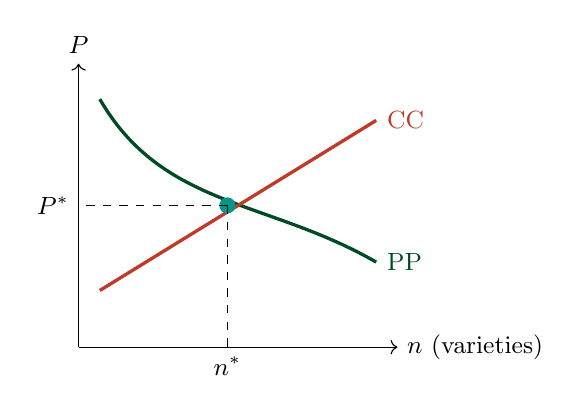
\begin{tikzpicture}[scale=0.9]
\draw[->] (0,0) -- (4.5,0) node[right]{\small $n$ (varieties)};
\draw[->] (0,0) -- (0,4) node[above]{\small $P$};
% PP: downward sloping
\draw[UNBCDark,very thick] (0.3,3.5) to[out=-60,in=150] (4.2,1.2) node[right]{\small PP};
% CC: upward sloping
\draw[AccentRed,very thick] (0.3,0.8) -- (4.2,3.2) node[right]{\small CC};
% Equilibrium
\filldraw[AccentTeal] (2.1,2.0) circle(3pt);
\draw[dashed] (2.1,2.0) -- (0,2.0) node[left]{\small $P^*$};
\draw[dashed] (2.1,2.0) -- (2.1,0) node[below]{\small $n^*$};
\end{tikzpicture}
\end{column}
\end{columns}
\end{frame}

\begin{frame}{How Trade Affects the Krugman Equilibrium}
\begin{columns}
\begin{column}{0.52\textwidth}
\textbf{Before trade}: market size = $S$ (Home only).\\[0.3em]
\textbf{After trade}: market size = $S + S^*$ (Home + Foreign).\\[0.3em]
\textbf{Effect on CC curve}:
\[P = c + \frac{n \cdot F}{S + S^*}\]
CC shifts \textbf{down}: at each $n$, break-even price is lower (more output per firm amortises $F$).\\[0.3em]
\textbf{Effect on PP curve}: no change (markup depends on $n$ only).\\[0.3em]
\textbf{New equilibrium}: lower $P$, higher $n$.
\end{column}
\begin{column}{0.45\textwidth}
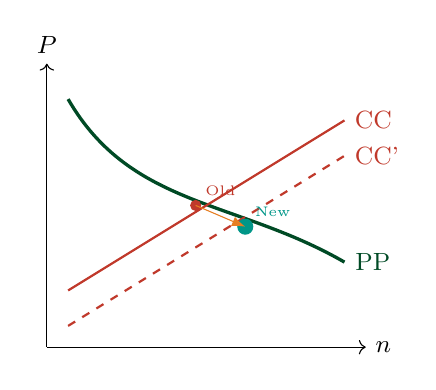
\begin{tikzpicture}[scale=0.9]
\draw[->] (0,0) -- (4.5,0) node[right]{\small $n$};
\draw[->] (0,0) -- (0,4) node[above]{\small $P$};
% PP
\draw[UNBCDark,very thick] (0.3,3.5) to[out=-60,in=150] (4.2,1.2) node[right]{\small PP};
% Old CC
\draw[AccentRed,thick] (0.3,0.8) -- (4.2,3.2) node[right]{\small CC};
% New CC (shifted down)
\draw[AccentRed,thick,dashed] (0.3,0.3) -- (4.2,2.7) node[right]{\small CC'};
% Old eq
\filldraw[AccentRed] (2.1,2.0) circle(2pt) node[above right]{\tiny Old};
% New eq
\filldraw[AccentTeal] (2.8,1.7) circle(3pt) node[above right]{\tiny New};
\draw[-{Latex},AccentOrange] (2.1,2.0) -- (2.8,1.7);
\end{tikzpicture}
\end{column}
\end{columns}
\end{frame}

\begin{frame}{Three Gains from Trade Under Monopolistic Competition}
\begin{columns}
\begin{column}{0.32\textwidth}
\begin{tcolorbox}[colback=UNBCDark!8,colframe=UNBCDark,title={\small\bfseries 1. Lower Prices},arc=2mm,left=1.5mm,right=1.5mm,top=0.8mm,bottom=0.8mm]
\small Larger market $\Rightarrow$ firms operate at larger scale $\Rightarrow$ lower $F/Q$ $\Rightarrow$ lower AC $\Rightarrow$ lower $P$.\\[0.3em]
Even if each firm's technology is unchanged, more output per firm lowers unit cost.
\end{tcolorbox}
\end{column}
\begin{column}{0.32\textwidth}
\begin{tcolorbox}[colback=AccentTeal!8,colframe=AccentTeal,title={\small\bfseries 2. More Variety},arc=2mm,left=1.5mm,right=1.5mm,top=0.8mm,bottom=0.8mm]
\small Net number of varieties available to consumers rises after trade. Each country specialises in different varieties but both countries' consumers gain access to the full range.\\[0.3em]
Consumers love variety (CES preferences).
\end{tcolorbox}
\end{column}
\begin{column}{0.32\textwidth}
\begin{tcolorbox}[colback=AccentBlue!8,colframe=AccentBlue,title={\small\bfseries 3. Pro-Competitive},arc=2mm,left=1.5mm,right=1.5mm,top=0.8mm,bottom=0.8mm]
\small More competition from foreign varieties lowers markups. Less efficient domestic firms exit. Surviving firms are larger and more productive (Melitz, 2003).\\[0.3em]
Aggregate productivity rises.
\end{tcolorbox}
\end{column}
\end{columns}
\vspace{0.3em}
\begin{canadex}[USMCA and Canadian Consumer Electronics]
  Removing tariffs on US electronics increased variety, lowered prices, and forced less efficient Canadian assemblers to exit --- all three gains occurred.
\end{canadex}
\end{frame}

\begin{frame}{Measuring Intra-Industry Trade: The Grubel-Lloyd Index}
\begin{columns}
\begin{column}{0.52\textwidth}
\begin{block}{Grubel-Lloyd (GL) Index}
\[\text{GL}_i = 1 - \frac{|X_i - M_i|}{X_i + M_i} \in [0,1]\]
where $X_i$ = exports of industry $i$, $M_i$ = imports of industry $i$.\\[0.3em]
$\text{GL} = 0$: pure inter-industry trade (only exports or only imports).\\
$\text{GL} = 1$: pure intra-industry trade (exports $=$ imports).
\end{block}
\end{column}
\begin{column}{0.45\textwidth}
\begin{adjustbox}{max width=\columnwidth}
\begin{tabular}{lc}
\toprule
\textbf{Country pair} & \textbf{GL index}\\
\midrule
Canada -- USA & 0.72\\
Germany -- France & 0.85\\
USA -- Mexico & 0.61\\
Japan -- South Korea & 0.58\\
USA -- Bangladesh & 0.12\\
Germany -- Nigeria & 0.08\\
\bottomrule
\multicolumn{2}{l}{\tiny Source: OECD; based on SITC 2-digit}
\end{tabular}
\end{adjustbox}
\begin{insight}{Pattern}
  High GL between similar rich countries; low GL between dissimilar countries (North-South trade follows H-O, not Krugman).
\end{insight}
\end{column}
\end{columns}
\end{frame}

\begin{frame}{Figure 7-1: External Economies and Market Equilibrium}
\begin{columns}
\begin{column}{0.54\textwidth}
\FIGH[0.96]{figures/slide15_img01.PNG}
\end{column}
\begin{column}{0.43\textwidth}
\textbf{What this figure shows:}
\begin{itemize}\small
  \item \textbf{Downward-sloping AC curve}: as industry output rises, external EoS reduce per-firm costs.
  \item \textbf{Demand curve}: downward sloping as usual.
  \item \textbf{Equilibrium}: price $= $ AC (zero profit); quantity at intersection.
  \item Key: the AC curve here is an \emph{industry-level} relationship --- individual firms are small and competitive, but the cluster lowers costs for all.
  \item This differs from internal EoS where one firm captures all cost savings.
\end{itemize}
\end{column}
\end{columns}
\end{frame}

\begin{frame}{Figure 7-2: External Economies Before Trade}
\begin{columns}
\begin{column}{0.54\textwidth}
\FIGH[0.96]{figures/slide17_img01.PNG}
\end{column}
\begin{column}{0.43\textwidth}
\textbf{Reading Figure 7-2:}
\begin{itemize}\small
  \item Shows two countries (Home and Foreign) with \emph{identical} external EoS AC curves.
  \item \textbf{Before trade}: each country produces at its domestic equilibrium.
  \item If Home has a \emph{larger industry} (due to history), Home operates at a lower AC.
  \item \textbf{Path dependence}: the country that had a head start maintains cost advantage --- even if technologies are identical.
  \item Trade with the larger industry may drive out the smaller one --- even if the smaller could have been equally efficient.
\end{itemize}
\begin{insight}{Policy Implication}
  First-mover advantage justifies infant-industry protection (cautiously).
\end{insight}
\end{column}
\end{columns}
\end{frame}

\begin{frame}{Figure 7-3: Trade and Prices with External Economies}
\begin{columns}
\begin{column}{0.54\textwidth}
\FIGH[0.96]{figures/slide21_img01.PNG}
\end{column}
\begin{column}{0.43\textwidth}
\textbf{What this figure shows:}
\begin{itemize}\small
  \item After trade, the country with the \textbf{larger} industry can produce at lower cost and supplies the world market.
  \item The smaller industry may be \textbf{driven out} entirely (complete specialisation due to EoS, not comparative advantage).
  \item The world price settles at the large-country's AC curve.
  \item Countries can become ``locked in'' to comparative advantage based on historical scale, not current productivity.
\end{itemize}
\begin{discuss}
  Should Canada protect its steel industry to build scale, or let the market decide? What does this figure suggest?
\end{discuss}
\end{column}
\end{columns}
\end{frame}

\begin{frame}{Industrial Clusters: Why Industries Agglomerate}
\begin{columns}
\begin{column}{0.52\textwidth}
\textbf{Three sources of external economies (Marshall, 1890):}\\[0.3em]
\textbf{1. Thick labour markets:}\\
A large pool of specialised workers reduces search costs and allows better job-worker matching. Both firms and workers benefit.\\[0.3em]
\textbf{2. Specialised suppliers:}\\
A cluster attracts specialised input suppliers (legal, financial, engineering services) that are not viable in smaller markets.\\[0.3em]
\textbf{3. Knowledge spillovers:}\\
Ideas and best practices flow more easily through face-to-face interaction. Proximity facilitates R\&D collaboration.
\end{column}
\begin{column}{0.45\textwidth}
\FIGH[0.95]{figures/slide25_img01.PNG}
\end{column}
\end{columns}
\end{frame}

\begin{frame}{Figure 7-4: The Importance of Established Advantage}
\begin{columns}
\begin{column}{0.54\textwidth}
\FIGH[0.96]{figures/slide25_img01.PNG}
\end{column}
\begin{column}{0.43\textwidth}
\textbf{What this figure shows:}
\begin{itemize}\small
  \item A country that establishes a cluster early enjoys a \textbf{self-reinforcing cost advantage}.
  \item Even if another country could potentially achieve lower costs at the same scale, it cannot profitably enter as long as the established cluster is large.
  \item The established advantage \emph{persists} over time --- historical accidents (where the first firm located) determine long-run industry geography.
  \item This is \textbf{path dependence}: history matters for economic geography.
\end{itemize}
\begin{canadex}
  Hollywood (film), Silicon Valley (tech), Waterloo (BlackBerry ecosystem), Vancouver (mining finance): all persist due to established cluster advantages.
\end{canadex}
\end{column}
\end{columns}
\end{frame}

\begin{frame}{Figure 7-5: External Economies and Potential Losses from Trade}
\begin{columns}
\begin{column}{0.54\textwidth}
\FIGH[0.96]{figures/slide29_img01.PNG}
\end{column}
\begin{column}{0.43\textwidth}
\textbf{What this figure shows:}
\begin{itemize}\small
  \item In some cases, trade can \textbf{harm} a country even with external EoS.
  \item If the foreign country has a larger cluster and lower AC, trade shifts all production there.
  \item The home country loses its entire industry.
  \item If the home industry \emph{could have been} viable at larger scale, this is a genuine welfare loss from trade.
  \item This provides the strongest theoretical case for infant-industry protection --- but the practical challenge remains: how do governments know which industries have this potential?
\end{itemize}
\end{column}
\end{columns}
\end{frame}

\begin{frame}{Policy Implications of Economies of Scale}
\begin{columns}
\begin{column}{0.52\textwidth}
\textbf{The case for industrial policy based on EoS:}
\begin{itemize}
  \item External EoS create a genuine market failure: firms cannot internalise industry-wide learning benefits.
  \item Path dependence means historical accidents determine industry location --- not efficiency.
  \item Temporary protection can allow a domestic industry to reach scale.
\end{itemize}
\vspace{0.3em}
\textbf{Counter-arguments:}
\begin{itemize}
  \item Governments rarely know which industries have large EoS.
  \item ``Temporary'' protection becomes permanent.
  \item Rent-seeking: protected industries lobby to stay protected.
  \item \textbf{Direct subsidies} are more efficient than tariffs (no consumer price distortion).
\end{itemize}
\end{column}
\begin{column}{0.45\textwidth}
\begin{canadex}[Bombardier C-Series: Vindicated Infant Industry?]
  Ottawa and Quebec subsidised Bombardier's C-Series aircraft development. Eventually sold to Airbus (now A220), which became globally successful.\\[0.3em]
  \textbf{Was the policy successful?}
  \begin{itemize}\small
    \item The product succeeded commercially.
    \item But: triggered US anti-dumping case (Boeing complaint, 300\% tariff).
    \item Bombardier had to give Airbus 50\%+ stake.
    \item Net fiscal cost to Canadian taxpayers: $>\$1$ billion.
  \end{itemize}
  \textbf{Verdict}: ambiguous at best.
\end{canadex}
\end{column}
\end{columns}
\end{frame}

\begin{frame}{Key Takeaways}
\begin{enumerate}
  \item \textbf{EoS and product differentiation} explain intra-industry trade between similar countries.
  \item \textbf{Krugman model}: trade expands market size, lowers prices (via scale), increases variety, and promotes competition --- three distinct gains.
  \item \textbf{Grubel-Lloyd index}: measures IIT; highest between similar rich countries.
  \item \textbf{External economies} create industrial clusters with path dependence --- historical accidents determine industry geography.
  \item \textbf{Potential losses from trade} with EoS provide a case for industrial policy, but practical challenges are severe.
  \item \textbf{Internal EoS} lead to imperfect competition --- a more complex analysis covered in advanced courses.
\end{enumerate}
\begin{block}{Next: Chapter 9 --- Instruments of Trade Policy}
  Tariffs, quotas, and their welfare effects.
\end{block}
\end{frame}

\end{document}
